\documentclass[compress]{beamer}
\usecolortheme{default}

\usepackage{lmodern, epstopdf, multirow, array, setspace, bbm, tcolorbox, pbox, bm, mathtools, tikz}
\usepackage[T1]{fontenc}

\setbeamertemplate{frametitle}[default][center]
\setbeamertemplate{footline}{\hfill \insertframenumber/\inserttotalframenumber\hspace*{5pt}\vspace{5pt}}
\setbeamertemplate{navigation symbols}{}

\newlength{\wideitemsep}
\setlength{\wideitemsep}{\itemsep}
\addtolength{\wideitemsep}{4pt}
\let\olditem\item
\renewcommand{\item}{\setlength{\itemsep}{\wideitemsep}\olditem}
\setlength{\leftmargini}{12pt}
\setlength{\leftmarginii}{14pt}
\setbeamertemplate{itemize/enumerate subbody begin}{\vspace{6pt}}
\setbeamertemplate{itemize item}[circle]
\setbeamertemplate{enumerate item}[circle]
\setbeamertemplate{enumerate subitem}[default]

\setbeamercolor{alerted text}{fg=blue}
\setbeamersize{text margin left=1.5em,text margin right=1.5em}

\tcbset{
    colback=white,
    colframe=black,
    coltext=black,
    coltitle=blue,
    colbacktitle=white,
    boxrule=1pt,
    titlerule=0pt,
    toptitle=4pt,
    top=2pt
}

\newenvironment{changemargin}[2]{% 
  \begin{list}{}{% 
    \setlength{\topsep}{0pt}% 
    \setlength{\leftmargin}{#1}% 
    \setlength{\rightmargin}{#2}% 
    \setlength{\listparindent}{\parindent}% 
    \setlength{\itemindent}{\parindent}% 
    \setlength{\parsep}{\parskip}% 
  }% 
  \item[]}{\end{list}}
  
\newenvironment{defn}{%
  \begin{tcolorbox}[title={Definition}]%
  }{\end{tcolorbox}}
  
\newenvironment{prop}[1]{%
  \begin{tcolorbox}[title={Proposition #1}]%
  }{\end{tcolorbox}}
  
\newcommand{\cit}[1]{{\footnotesize \textcolor[rgb]{0.5,0,0}{#1}}}

% Font size for code listings (verbatim blocks); reset with \normalsize
\newcommand{\codesize}{\fontsize{7}{8.5}\selectfont}

\newcommand{\slidesetup}[1]{%
  \title{#1}%
  \subtitle{\texorpdfstring{\vspace{0.3\baselineskip}}{} {\small This version: \today}}%
  \author[Mikkel Plagborg-Moller]{ECMA 31150, Spring 2026 \texorpdfstring{\\[0.5ex]}{} University of Chicago \texorpdfstring{\\[0.5ex]}{} Department of Economics \texorpdfstring{\\[4ex]}{} Mikkel Plagborg-Moller}%
  \date{}%
}

% \circleoverlay[options]{text}
% Draws a red circle with a text box nearby on a tikz overlay.
% Options (with defaults):
%   cx=0cm, cy=0cm      - circle center (shift from page center)
%   r=1cm               - circle radius
%   tx=0cm, ty=0cm      - text box offset from circle center
%   text anchor=east    - anchor of text node (east = text left, west = text right)
%   font=\normalsize    - font size for text
\pgfkeys{
  /circleoverlay/.cd,
  cx/.store in=\cocx, cx=0cm,
  cy/.store in=\cocy, cy=0cm,
  r/.store in=\cor, r=1cm,
  tx/.store in=\cotx, tx=0cm,
  ty/.store in=\coty, ty=0cm,
  text anchor/.store in=\cotextanchor, text anchor=east,
  font/.store in=\cofont, font=\normalsize,
}
\newcommand{\circleoverlay}[2][]{%
  \pgfkeys{/circleoverlay/.cd, cx=0cm, cy=0cm, r=1cm, tx=0cm, ty=0cm, text anchor=east, font=\normalsize, #1}%
  \pgfmathsetlengthmacro{\circlediameter}{2*\cor}%
  \node[draw=red, line width=2pt, circle, minimum size=\circlediameter, inner sep=0pt]
    (tmpcirc) at ([xshift=\cocx,yshift=\cocy]current page.center) {};%
  \node[anchor=\cotextanchor, fill=white, draw=red, text=red, inner sep=4pt, align=left, font=\cofont]
    at ([xshift=\cotx,yshift=\coty]tmpcirc.center) {#2};%
}

\DeclareMathOperator*{\argmax}{argmax}
\DeclareMathOperator*{\argmin}{argmin}
\DeclareMathOperator{\diag}{diag}
\DeclareMathOperator{\var}{Var}
\DeclareMathOperator{\cov}{Cov}
\DeclareMathOperator{\corr}{Corr}
\DeclareMathOperator{\lrv}{LRV}


\slidesetup{Forecasting with stationary models I}

\begin{document}
\frame{
\maketitle
}

\frame{
\frametitle{Plan for this slide deck}
\begin{enumerate}
\item What is time series analysis?
\item Definition of time series
\item Stationarity
\item Serial correlation, autocorrelation function
\end{enumerate}
}

\frame{
\frametitle{What is time series analysis?}
\begin{itemize}
\item Time series: data with \emph{time ordering}.
\item Observations often not i.i.d.\ or even uncorrelated over time. ``Random sampling'' from super-population not relevant.
\item Topics that receive more emphasis in time series analysis than in cross-sectional econometrics:
\begin{itemize}
\item Forecasting (prediction).
\item Small sample sizes.
\item Strong dependence over time.
\item Unstable models over time.
\item Data always observational. Must look hard for ``natural experiments''.
\item Theory (structural models) to guide/complement causal inference.
\end{itemize}
\end{itemize}
}

\frame{
\begin{figure}
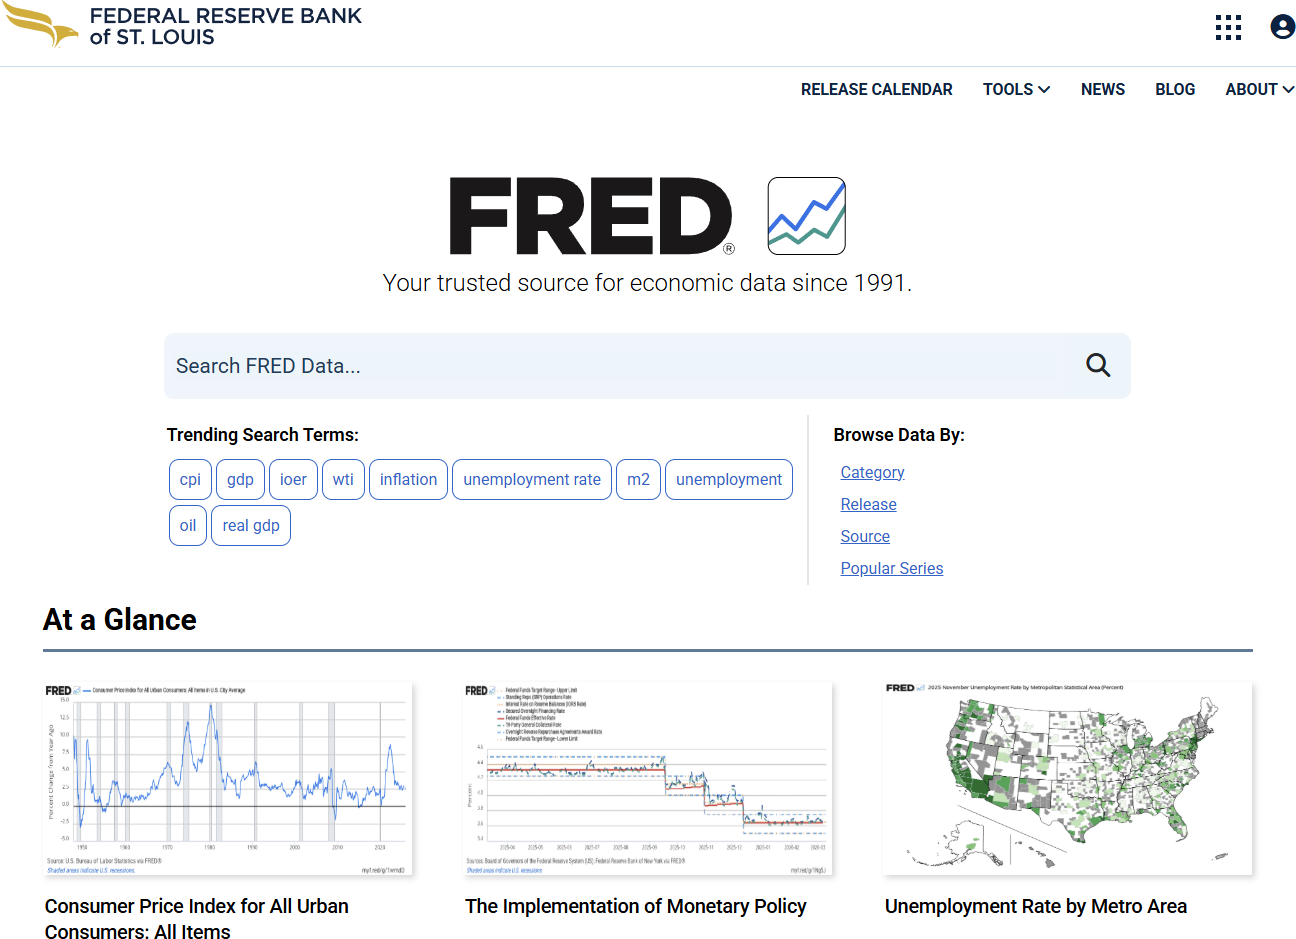
\includegraphics[width=0.9\linewidth]{fig/fred.png} \\
\medskip
\url{https://fred.stlouisfed.org}
\end{figure}
}

\frame{
\begin{figure}
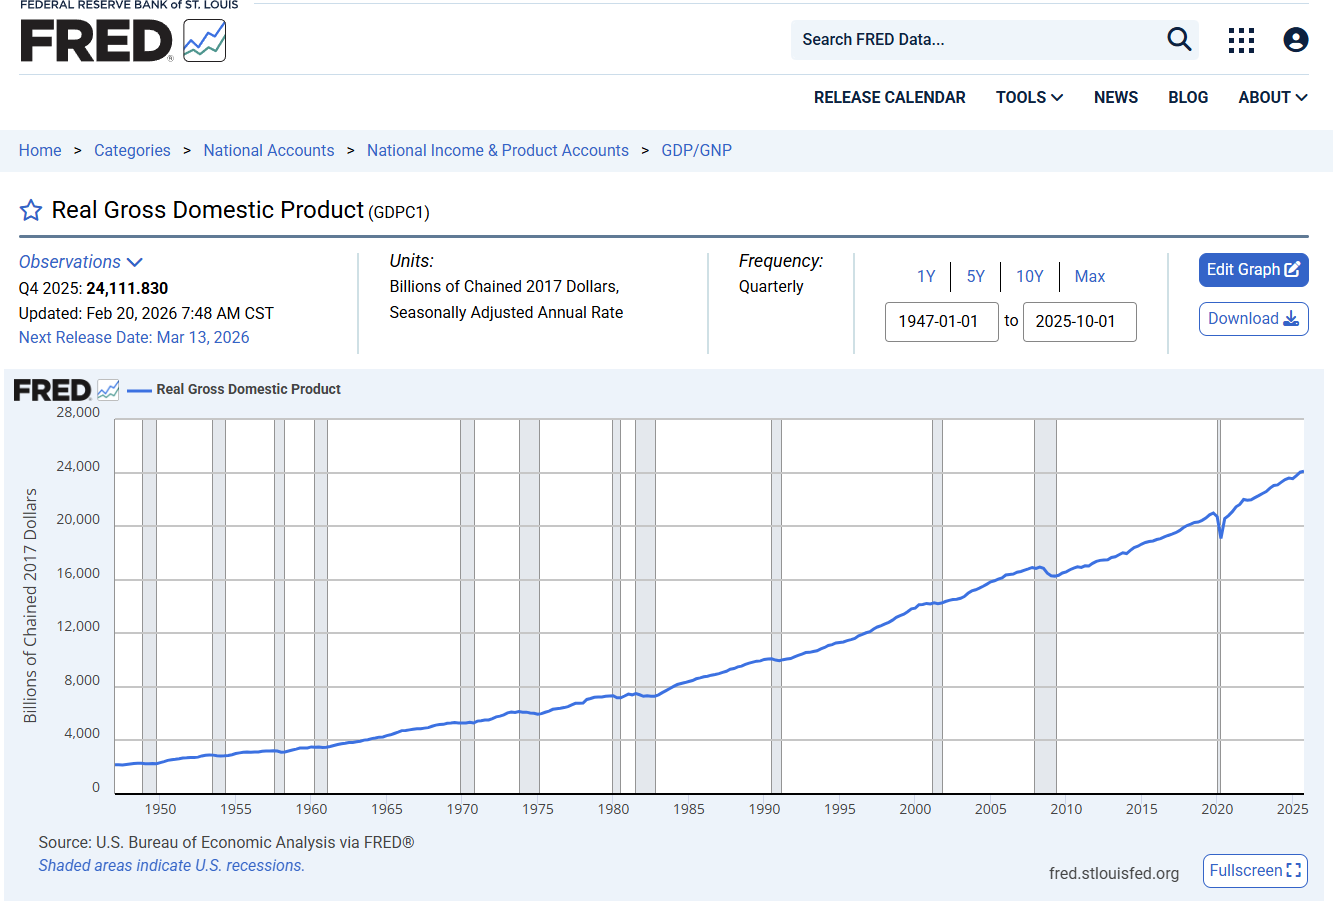
\includegraphics[width=\linewidth]{fig/fred_rgdp.png}
\end{figure}
\begin{tikzpicture}[remember picture, overlay]
\only<2>{
  \circleoverlay[cx=5cm, cy=0.2cm, tx=-1.2cm]{Forecasting: what next?}
}
\only<3>{
  \circleoverlay[cx=-4.7cm, cy=-2cm, text anchor=west, tx=1.2cm, ty=1cm]{Small sample: post-WW2 \\ $\sim 315$ quarters at best}
}
\end{tikzpicture}
}

\frame{
\begin{figure}
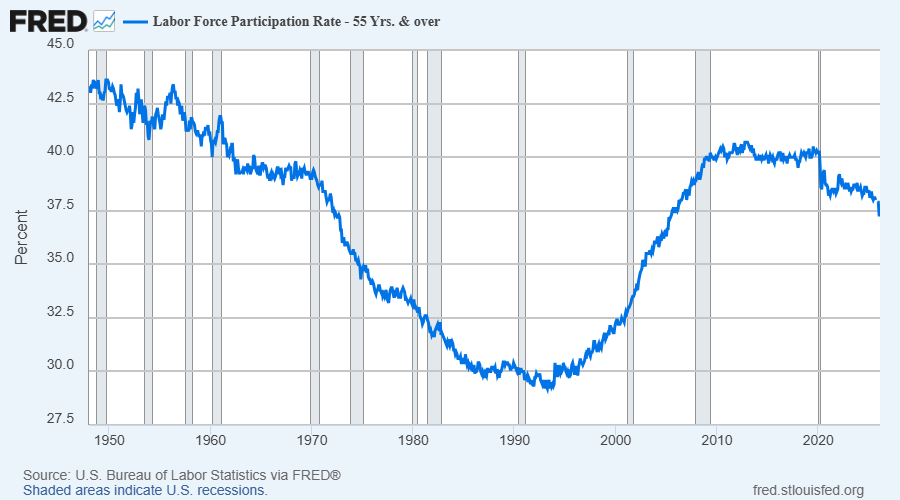
\includegraphics[width=\linewidth]{fig/fred_lfpr.png}
\end{figure}
\begin{tikzpicture}[remember picture, overlay]
\only<2>{
  \circleoverlay[cy=1cm, r=4cm, text anchor=west, tx=1cm, ty=2cm]{Highly persistent}
}
\only<3>{
  \circleoverlay[cx=4.7cm, cy=1.5cm, tx=-1.2cm]{Break?}
}
\end{tikzpicture}
}

\frame{
\begin{figure}
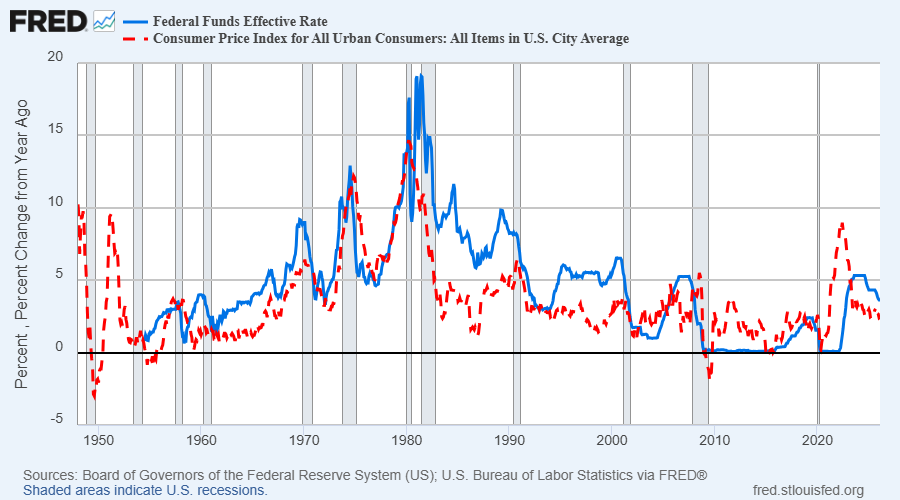
\includegraphics[width=\linewidth]{fig/fred_fedfunds_cpi.png} \\
\medskip
Causation vs.\ correlation: can the Federal Reserve control inflation? \\
\medskip
Dearth of experiments. Policy-makers don't roll dice -- need theory!
\end{figure}
}

\frame{
\frametitle{Forecasting}
\begin{itemize}
\item The first part of this course will not consider \textbf{causal} questions: does $X$ affect $Y$ if we hold \emph{everything else constant}?
\begin{itemize}
\item We'll get back to these later -- don't worry!
\end{itemize}
\item Instead we will be concerned with \textbf{forecasting} (prediction): what is our best guess of the future value of $Y$, given what we observe up to the present?
\item A variable might be helpful for forecasting without being causally important.
\begin{itemize}
\item Example: the number of students carrying umbrellas to school in the morning is a good predictor of rainfall in the afternoon.
\end{itemize}
\item Forecasting is a key role of economists in industry + government.
\end{itemize}
}

\frame{
\begin{figure}
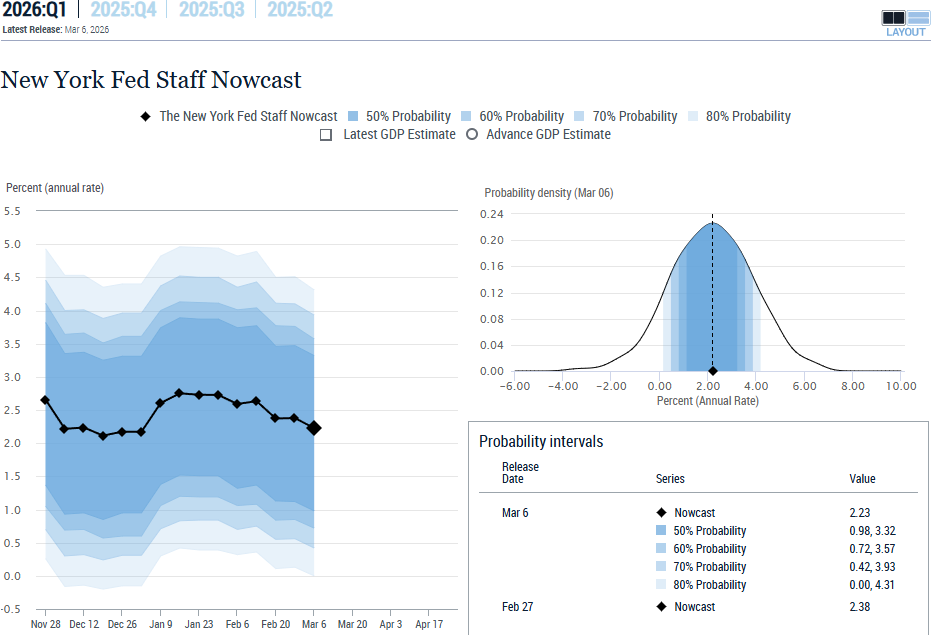
\includegraphics[width=0.9\linewidth]{fig/nyfed_nowcast1.png} \\
\medskip
\url{https://www.newyorkfed.org/research/policy/nowcast}
\end{figure}
}

\frame{
\begin{figure}
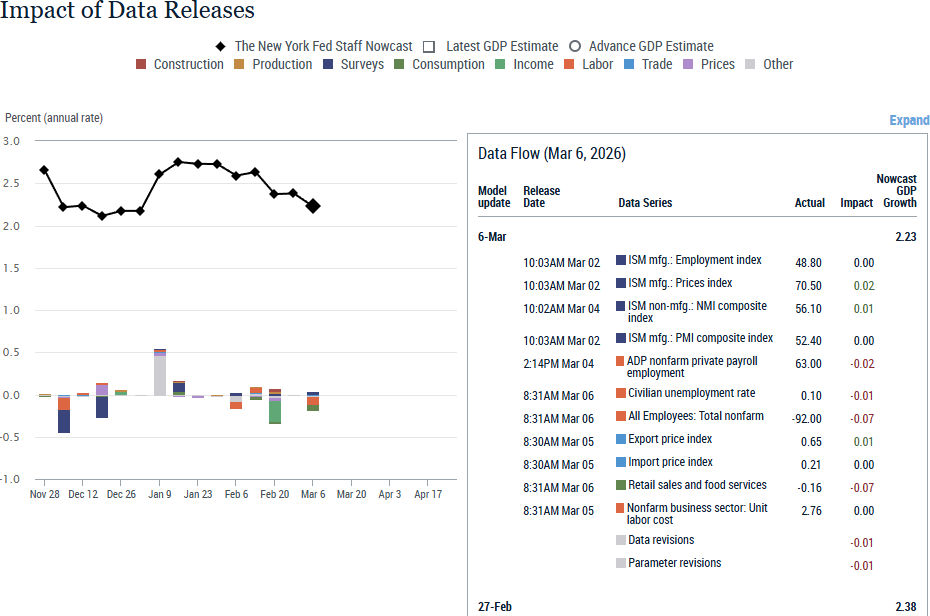
\includegraphics[width=0.9\linewidth]{fig/nyfed_nowcast2.png} \\
\medskip
There's a wealth of public data series to use as predictors -- but we will start by looking at small models and then expand from there.
\end{figure}
}

\frame{
\frametitle{Mathematical definition of a time series}
\begin{itemize}
\item A \textbf{time series} (or \textbf{stochastic process}) is a collection of random variables $y_1,y_2,y_3,\dots$ whose ordering matters.
\item We refer to the index $t$ in $y_t$ as ``time''.
\begin{itemize}
\item Could be measured in days, months, quarters, years, etc.
\end{itemize}
\item Being random variables, each $y_t$ can be viewed as a function of an outcome $\omega$ in some latent sample space $\Omega$: $y_t(\omega)$.
\begin{itemize}
\item Think of $\Omega$ as all possible histories of the world, and $\omega$ as one realization.
\end{itemize}
\item The time profile $y_1(\omega),y_2(\omega),y_3(\omega),\dots$ is a \textbf{sample path} (or \textbf{realization}) of the time series. Conceptually, we can imagine alternative histories of the world, with different $\lbrace y_t \rbrace$ paths.
\begin{itemize}
\item What if Napoleon had died from a stroke in 1802?
\item What if the Covid virus had mutated slightly differently?
\end{itemize}
\end{itemize}
}

\frame{
\frametitle{Autoregressive process}
\begin{itemize}
\item Consider a time series $\lbrace y_t \rbrace$ given by the recursive definition
\[y_t = \rho y_{t-1} + u_t,\quad \text{where}\quad u_t \overset{iid}{\sim} N(0,1) \quad \text{and}\quad y_0=0.\]
\item This is called an \textbf{autoregression} (depends on its own past value).
\item Think of $u_t$ as random ``\textbf{shocks}'' that affect the evolution of the process (e.g., good/bad harvest, arrival of technological innovation).
\begin{itemize}
\item To link with previous slide, $u_t$ is implicitly itself a function of some underlying outcome $\omega$, yielding the standard normal distribution.
\end{itemize}
\item Next slide: three simulated sample paths for $t=1,2,\dots,100$ and $\rho=0.95$.
\end{itemize}
}

\frame{
\begin{figure}
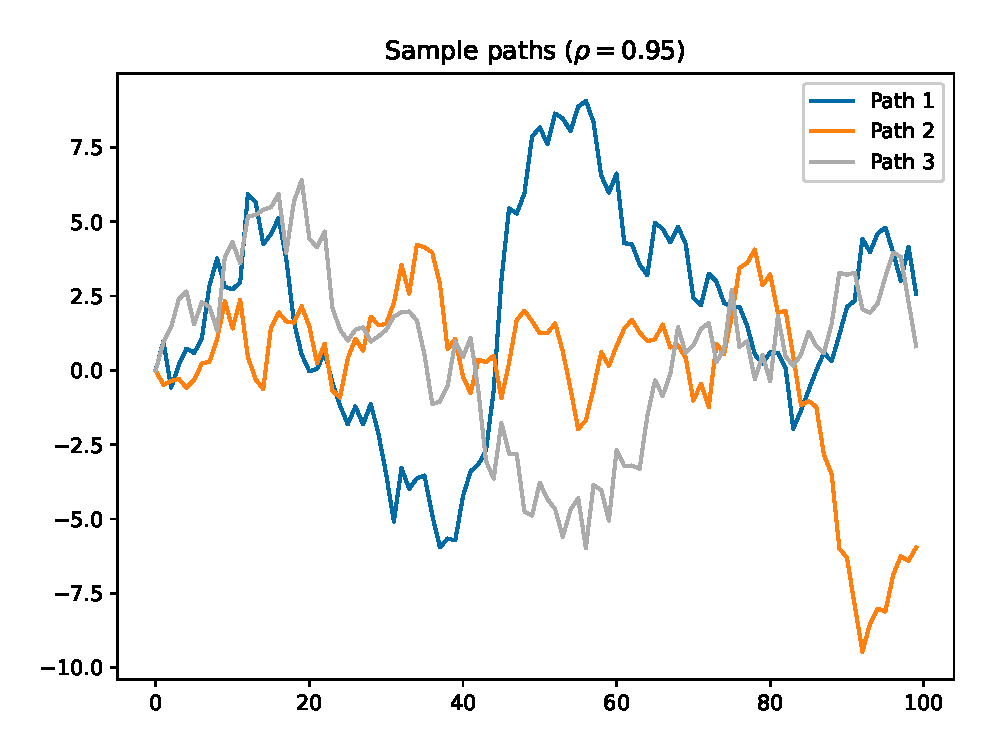
\includegraphics[width=0.9\linewidth]{fig/ar_sim.eps} \\
Each path is different, but they look deceptively like ``typical'' economic time series: persistent fluctuations, mixture of small+large movements
\end{figure}
}

\frame{
\begin{figure}
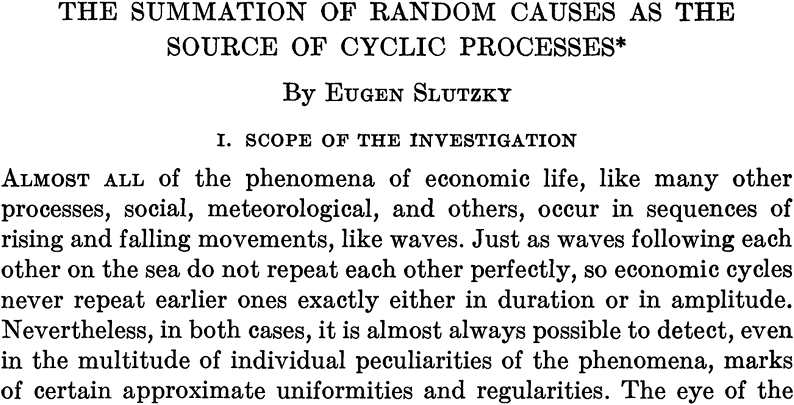
\includegraphics[width=0.7\linewidth]{fig/slutsky_paper.png} \\
\medskip
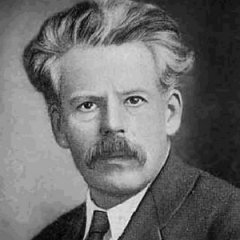
\includegraphics[width=0.3\linewidth]{fig/eugen_slutsky_photo.jpg}
\end{figure}
}

\frame{
\frametitle{Impulse-propagation paradigm}
\begin{itemize}
\item Slutsky (1927, previous slide), George Udny Yule (1927), and Ragnar Frisch (1933) developed the \textbf{impulse-propagation paradigm} for economic analysis.
\item Impulse: random, external shocks that hit the economy.
\item Propagation: the regular transmission mechanisms of the economy.
\begin{itemize}
\item E.g., income falls $\rightarrow$ consumers cut back spending $\rightarrow$ businesses cut investment $\rightarrow$ \dots
\end{itemize}
\item Hence, we get persistent cycles from irregular, unpredictable shocks.
\end{itemize}
\medskip
\begin{quotation}
If you hit a wooden rocking-horse with a club, the movement of the horse will be very different from that of the club. \\ \hfill --- {\upshape Ragnar Frisch, 1933}
\end{quotation}
}

\frame{
\frametitle{Stationarity}
\begin{itemize}
\item If we want to forecast, we need to make some kind of assumption that ``the future will be like the past''.
\end{itemize}
\medskip
\begin{quotation}
That the sun will not rise tomorrow is no less intelligible a proposition, and implies no more contradiction than the affirmation, that it will rise. \hfill --- {\upshape David Hume, 1748}
\end{quotation}
\medskip
\begin{itemize}
\item The starting point is the following (will relax later).
\item The time series $\lbrace y_t \rbrace$ is \textbf{(strictly) stationary} if for any integers $k,\ell$, the distribution of $(y_t,y_{t+1},\dots,y_{t+k})$ is the same as that of $(y_{t+\ell},y_{t+1+\ell},\dots,y_{t+k+\ell})$.
\begin{itemize}
\item The distribution of $(y_t,y_s)$ depends on $t,s$ only through $t-s$.
\end{itemize}
\item The \emph{realized shocks} make $y_t$ different from $y_s$ for $s \neq t$, but \emph{across histories of the world} each time point tends to behave the same (and similarly for each slice of consecutive time points).
\end{itemize}
}

\frame{
\frametitle{Non-stationarity}
\begin{itemize}
\item We'll talk at length about non-stationary models later.
\item Examples of non-stationarity:
\begin{itemize}
\item A discrete break in the structure of the time series: distribution of $y_t$ changes after the break.
\item A predictable trend in the series over time: average values are higher later in the sample than earlier.
\item Seasonality: e.g., January systematically different from February.
\end{itemize}
\item Example of structural break:
\[y_t = c_t + \rho y_{t-1} + u_t, \quad \text{where} \quad c_t = \begin{cases}
0 & \text{for } t < t^*, \\
1 & \text{for } t \geq t^*.
\end{cases}\]
\end{itemize}
}

\frame{
\begin{figure}
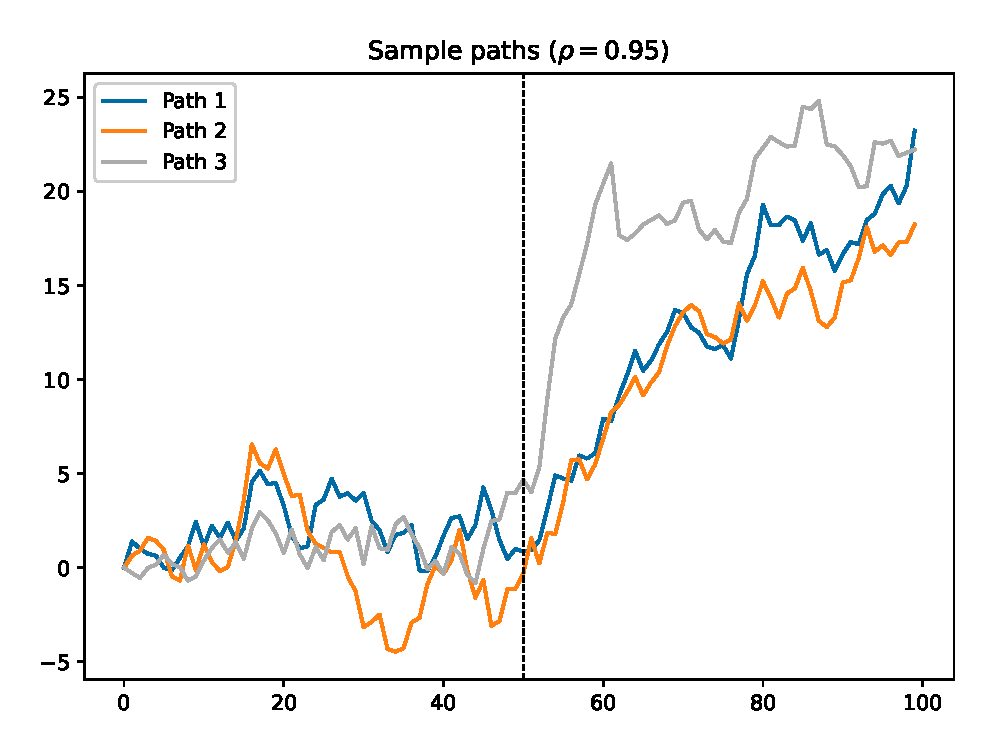
\includegraphics[width=0.9\linewidth]{fig/ar_sim_break.eps} \\
Break at time $t^*=50$
\end{figure}
}

\frame{
\begin{figure}
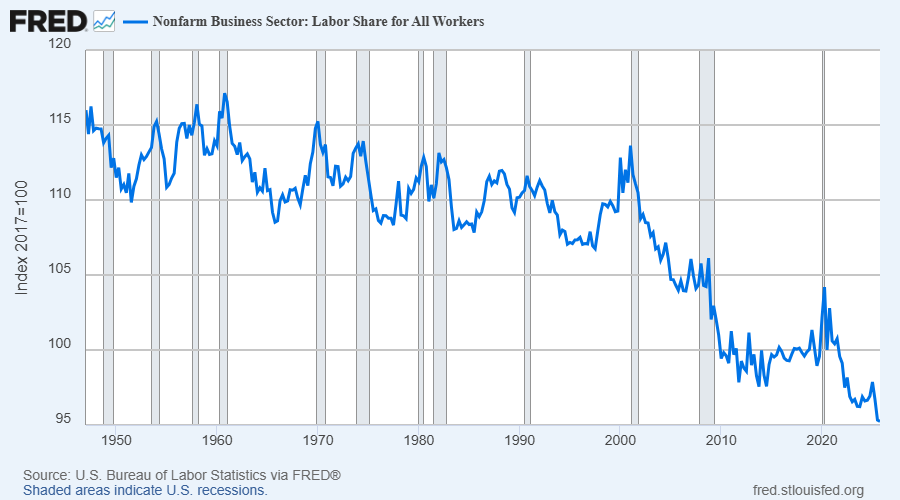
\includegraphics[width=\linewidth]{fig/fred_laborshare.png}
\end{figure}
\begin{tikzpicture}[remember picture, overlay]
\only<2>{
  \circleoverlay[r=2cm, cx=2.5cm, cy=1cm, text anchor=west, tx=1.2cm]{Break?}
}
\end{tikzpicture}
}

\frame{
\frametitle{Differencing and logs}
\begin{itemize}
\item If a time series does not look stationary, sometimes its \textbf{first differences} (changes) do:
\[\Delta y_t \equiv y_t - y_{t-1}.\]
\item Many economic time series look reasonably stationary in \emph{logged} first differences:
\[\Delta \log y_t \equiv \log y_t - \log y_{t-1}.\]
(In Econ, ``log'' always means natural logarithm.)
\item This is because $\log(1+z) \approx z$ for small $z$ (\alert{why?}), so
\[\Delta \log y_t \approx \frac{y_t-y_{t-1}}{y_{t-1}} = \frac{1}{100} \times (\text{\% change in } y_t),\]
and many economic series have fairly stable \emph{growth rates}.
\end{itemize}
}

\frame{
\begin{figure}
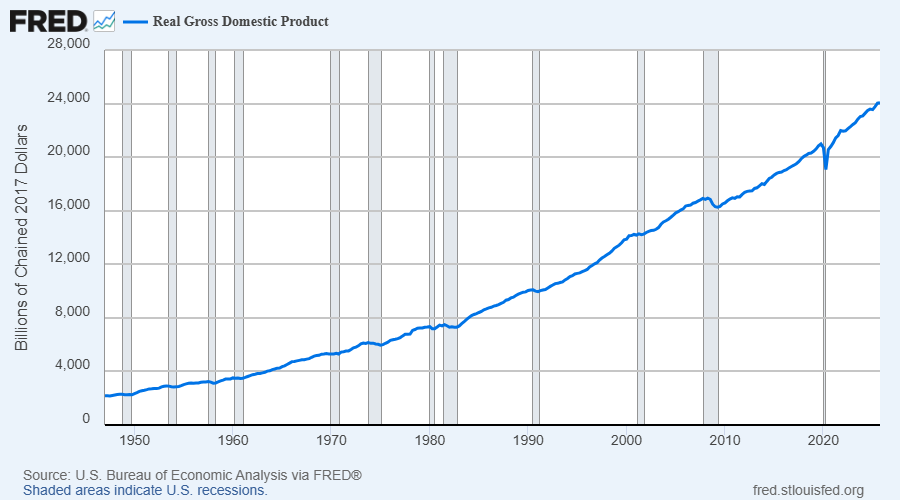
\includegraphics[width=0.9\linewidth]{fig/fred_gdpc1.png} \\
Real GDP in levels
\end{figure}
}

\frame{
\begin{figure}
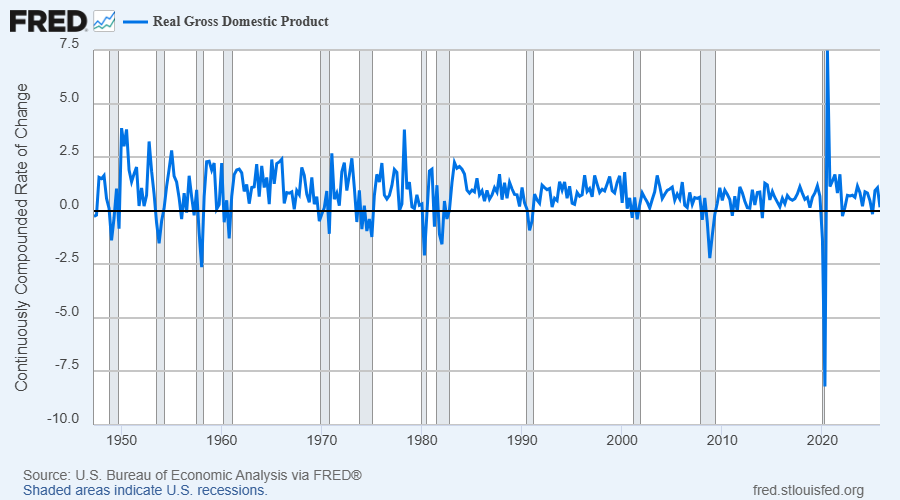
\includegraphics[width=0.9\linewidth]{fig/fred_gdpc1_dlog.png} \\
Log growth rate of real GDP (quarterly)
\end{figure}
}

\frame{
\frametitle{Lags and leads}
\begin{itemize}
\item Terminology:
\begin{itemize}
\item $y_{t-1}$ is the \textbf{lag} of $y_t$ (prior observation).
\item $y_{t-\ell}$ is the $\ell$-th lag of $y_t$ ($\ell$ periods prior).
\item $y_{t+1}$ is the \textbf{lead} of $y_t$ (next observation).
\item $y_{t+\ell}$ is the $\ell$-th lead of $y_t$ ($\ell$ periods after).
\end{itemize}
\item If we want to forecast, we need to know how $y_t$ is related to its lags $y_{t-1},y_{t-2},\dots$.
\end{itemize}
}

\frame{
\frametitle{Autocorrelations}
\begin{itemize}
\item Let's assume we have a stationary time series $\lbrace y_t \rbrace$.
\item Then $E(y_t)$, $\var(y_t)$, and $\cov(y_t,y_{t-\ell})$ do not depend on $t$ (for any integer $\ell$).
\item We call these the mean, variance, and \textbf{autocovariance} at \textbf{lag} $\ell$.
\item The function $\gamma(\ell) \equiv \cov(y_t,y_{t-\ell})$ is the \textbf{autocovariance function}.
\begin{itemize}
\item Note: $\gamma(0)=\var(y_t)$.
\end{itemize}
\item The function $\rho(\ell) \equiv \corr(y_t,y_{t-\ell}) = \frac{\gamma(\ell)}{\gamma(0)} \in [-1,1]$ is the \textbf{autocorrelation function (ACF)}.
\item The ACF satisfies $\rho(-\ell)=\rho(\ell)$.
\end{itemize}
}

\begin{frame}[fragile]
\frametitle{Sample autocorrelation function}
\begin{itemize}
\item Given data, we can estimate the autocorrelation in the obvious way:
\[\hat{\rho}(\ell) \equiv \frac{\sum_{t=\ell+1}^T (y_t-\bar{y})(y_{t-\ell}-\bar{y})}{\sum_{t=1}^T (y_t-\bar{y})^2},\]
where $\bar{y}$ is the sample average.
\begin{itemize}
\item The function $\hat{\rho}(\ell)$, $\ell \geq 1$, is sometimes called the \textbf{correlogram}.
\end{itemize}
\item Python:
\medskip
\begin{verbatim}
from statsmodels.tsa.stattools import acf
rho = acf(y, nlags=48)
\end{verbatim}
\end{itemize}
\end{frame}

\frame{
\begin{figure}
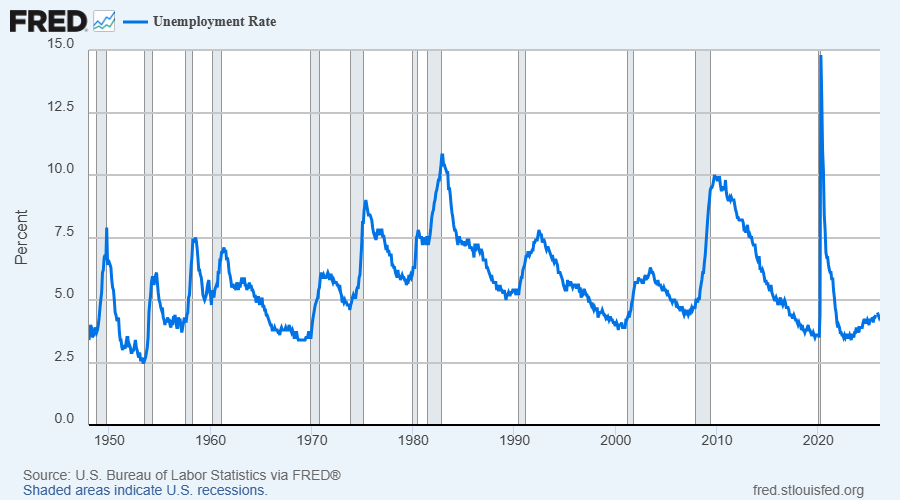
\includegraphics[width=0.9\linewidth]{fig/fred_unrate.png}
\end{figure}
}

\frame{
\begin{figure}
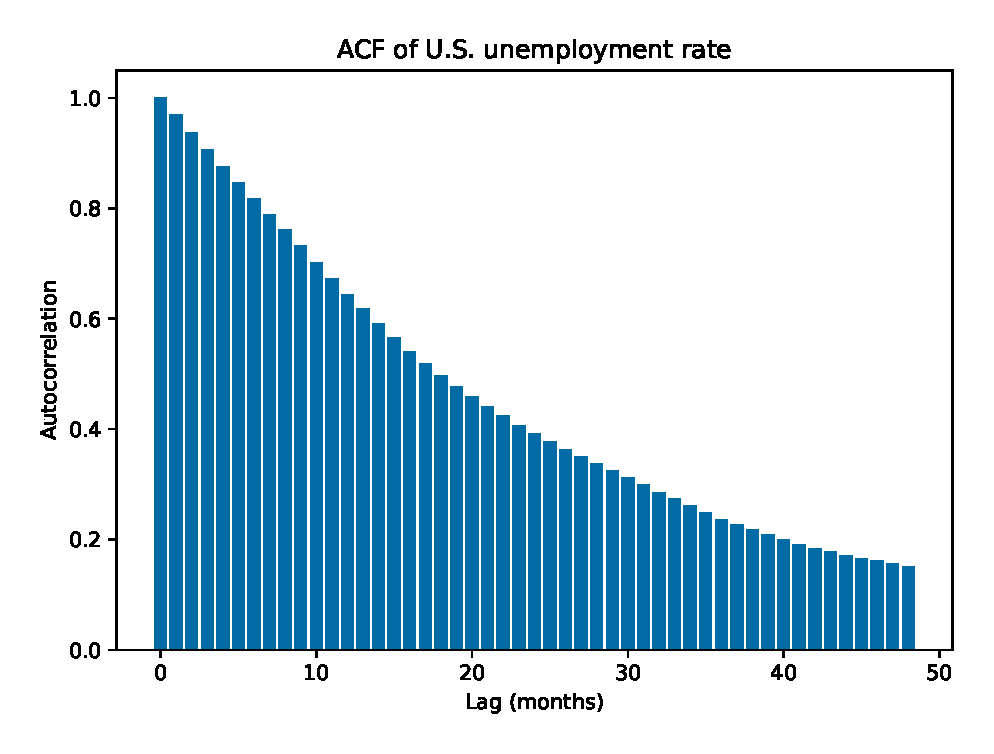
\includegraphics[width=0.9\linewidth]{fig/unrate_acf.eps} \\
$\hat{\rho}(\ell) > 0$ for $\ell=1,2,\dots$: the series is \textbf{positively serially correlated}. \\
\medskip
The persistence is quite strong. $\hat{\rho}(\ell)>0.2$ even after 3 years.
\end{figure}
}

\frame{
\frametitle{Covariance stationarity}
\begin{itemize}
\item We will often only be concerned with the first and second moments of time series (mean, autocovariances).
\item It then makes sense to work with the following weaker stationarity concept.
\item $\lbrace y_t \rbrace$ is \textbf{covariance stationary} if neither its mean nor its autocovariances depend on time.
\end{itemize}
\medskip
\[\text{strict stationarity} + \text{variance exists} \; \Longrightarrow \; \text{covariance stationarity}\]
\[\text{covariance stationarity} \;\; \not{\!\!\!\Longrightarrow} \;\; \text{strict stationarity}\]
}

\frame{
\frametitle{White noise}
\begin{itemize}
\item As a building block for more complicated dynamic models (next lectures), it's useful to define a process that is \emph{not} serially correlated.
\item A covariance stationary series $\lbrace y_t \rbrace$ is \textbf{white noise} if:
\begin{enumerate}
\item $E(y_t)=0$.
\item $\gamma(\ell)=0$ for $\ell \geq 1$ (\textbf{serially uncorrelated}).
\end{enumerate}
\item For a white noise process, there's no correlation between the \emph{level} of the series at time $t$ and the level at any other time $s$.
\begin{itemize}
\item But there could be serial correlation in $|y_t|$, say.
\end{itemize}
\item Special case of white noise process: martingale difference sequence (next slide).
\end{itemize}
}

\frame{
\frametitle{Martingale difference sequence}
\begin{itemize}
\item A series $\lbrace y_t \rbrace$ is called a \textbf{martingale} with respect to the \textbf{filtration} (sequence of information sets) $\lbrace \mathcal{F}_t \rbrace_t$ if:
\begin{enumerate}
\item $y_t \in \mathcal{F}_t$ for all $t$ (\textbf{adapted} to the filtration).
\item $E[y_t \mid \mathcal{F}_{t-1}] = y_{t-1}$ (best forecast = no change).
\end{enumerate}
\item Typically, $\mathcal{F}_t = \sigma(y_t,y_{t-1},y_{t-2},\dots)$, the information generated by past data.
\item A series $\lbrace y_t \rbrace$ is called a \textbf{martingale difference sequence} (MDS) if it's adapted to $\mathcal{F}_t$ and
\[E[y_t \mid \mathcal{F}_{t-1}] = 0.\]
\vspace{-1.5\baselineskip}
\begin{itemize}
\item Real-world example: stock returns (efficient markets).
\end{itemize}
\item If $\lbrace y_t \rbrace$ is a martingale, then $\Delta y_t$ is a MDS.
\end{itemize}
}

\frame{
\frametitle{Martingale difference sequence: example}
\begin{figure}
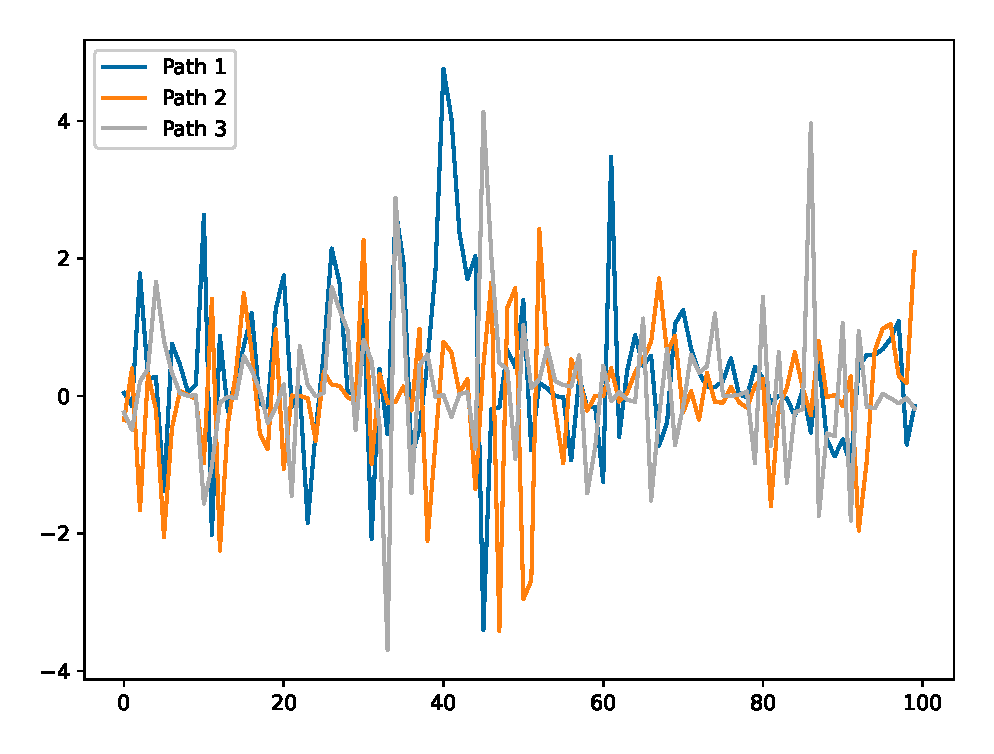
\includegraphics[width=0.65\linewidth]{fig/mds.eps}
\end{figure}
\[y_t = |u_{t-1}|u_t,\quad u_t \overset{iid}{\sim} N(0,1)\]
\alert{Exercise:} show that $\lbrace y_t \rbrace$ is a MDS. But it's not independent over time: $\cov(\log|y_t|,\log|y_{t-1}|) = \var(\log|u_t|) \neq 0$.
}

\frame{
\frametitle{Relationship between concepts}
\begin{itemize}
\item \alert{Exercise:} prove that for a time series $\lbrace y_t \rbrace$ with mean zero and finite variance that is constant through time,
\[\text{i.i.d.} \quad \Longrightarrow \quad \text{MDS} \quad \Longrightarrow \quad \text{white noise}.\]
\item Here the MDS is wrt.\ the natural filtration $\mathcal{F}_t = \sigma(y_t,y_{t-1},y_{t-2},\dots)$.
\end{itemize}
}

\frame{
\frametitle{What did we learn?}
\begin{itemize}
\item Mathematical definition of time series
\item Example: AR process
\item Stationarity, differencing
\item Concepts related to serial correlation
\begin{itemize}
\item ACF: population, sample
\item White noise, martingale difference sequence
\end{itemize}
\end{itemize}
}

\frame{
\frametitle{Looking ahead}
\begin{itemize}
\item How to model time series dependence?
\item Autoregressive model
\begin{itemize}
\item Stationarity
\item Moments
\item Forecasting
\item Choice of lag length
\end{itemize}
\end{itemize}
}

\end{document}
